
\section{Accelerator Modifications: Rebunching protons at a higher RF frequency}
\label{RF}

The proton bunch must have as small a duration as possible in order to
select neutrino energies based on position/time of arrival at the
detector (see section 9). This section describes one example of how to
create longitudinally thin proton bunches with on the order of 100 ps
time width in the Fermilab Main Injector (MI) with minimal changes to
the existing accelerating infrastructure. Outputs from a simulation of
this re-bunching scheme are presented.


\subsection{Properties of the present main injector proton bunch}
The main injector is filled with protons from the booster ring which
injects \textit{batches} of 8 GeV protons. Each batch contains 84 RF
\textit{buckets} at 53.1MHz. The main injector ring has space to hold
7 batches, or 588 buckets, but is only filled with 6 batches leaving an 
\textit{abort gap} of 84 buckets for the \textit{kicker} which sends the
 beam into the NuMI target. Every 1.2 s (referred to below as the \textit{cycle
  time}), the kicker is engaged and 6 batches of protons are extracted
into the NuMI target downstream, creating about 10 $\mu$s of bunched
neutrino beam.

The longitudinal position of a proton in the bunch changes depending
on its momentum. Each proton in the bunch occupies a point in the
phase space of RF phase $\phi$ (or longitudinal location in the bunch)
and momentum relative to the synchronous particle momentum, $\delta =
\mathrm{d}p/p_0$.

Each main injector RF bucket is about 20 ns long but the protons occupy a small 
fraction of the bucket. Protons from the booster enter the main injector with a
$(\phi, \delta)$ phase-space area of about 0.2 eVs (95\% of particles). Each MI bunch
is a combination of two slip-stacked booster bunches, which after acceleration leads to
about 0.7-1 eVs of phase space area. This proton bunch is
non-gaussian with an RMS time-width of about 900 ps (cite). At 1 eVs, this implies that 

\begin{equation}
\mathrm{d}p_{rms} \simeq \frac{1 [\texttt{eVs}]}{6\pi t_{rms}}  \simeq 37 \quad \texttt{MeV}
\end{equation}

or a $\delta$ of $3\times 10^{-4}$. An attempt to generate this initial particle distribution
is used in the simulations below and is shown in red in figure \ref{fig:bunch_distributions}.


\subsection{Higher frequency RF structure and hardware}

The main injector proton bunch will need to be re-bunched into a
roughly 10-times higher frequency RF structure in order to achieve a
goal of 100 ps bunch width for doing stroboscopic neutrino physics. An
insertion of only one such RF cavity into the existing ring would
allow for higher frequency re-bunching.

The company \textit{Research Instruments} commercially produces
superconducting RF cavities at 500MHz for use in electron storage
rings like the Canadian Light Source
\cite{nsls-cavity}\cite{cls_stampe}\cite{research_instruments}. These
cavities are designed to operate at 2 MV RF amplitude which is within the
voltage amplitudes supplied to the present main injector cavities.
 The commercial availability of such cavities is encouraging,
as this cavity could be used in prototyping and early testing of the
re-bunching sequence. 


\subsection{Example of a rebunching procedure in the Fermilab Main Injector}

A simulation has been written to study the following properties of a
rebunching procedure: the ramp-down/ramp-up functions for re-bunching
at a higher frequency, the final RMS bunch width, and the total
additional time needed to re-bunch. These quantities will place
constraints on the re-bunching cavity as well as shed light on the
impact to neutrino physics for a given loss in total POT.

\subsubsection{Simulation equations}

The simulation presented uses the paraxial approximation for
longitudinal synchrotron motion in a circular accelerator:

\begin{equation}
\dot{\delta} = \frac{\omega_0 e V_{rf}}{\beta ^2 W}\sin(\phi) 
\end{equation}
\begin{equation}
\dot{\phi} = -2\pi h \eta \delta \omega_0
\end{equation}

where $\omega_0$ is the RF cavity frequency ($\phi = \omega_0 t$),
$\delta$ is the $\mathrm{d}p/p_0$ momentum fraction relative to the
synchronous reference momentum $p_0$, $V(\phi) = V_{rf}\sin(\phi)$ is
the RF voltage function with amplitude $V_{rf}$, $\beta$ is the
relativistic velocity of the protons, $W = E + m_p$ where $m_p$ is the
mass of the proton and $E$ is the design energy of the beam, $h$ is
the harmonic number, and $\eta$ is the phase slip factor.

A first order discrete approximation of these equations can be used to
calculate particle dynamics in $(\phi, \delta)$ phase-space

\begin{equation}
\delta_{n+1} = \delta_n +  \frac{e V_{rf}}{\beta ^2 W}\sin(\phi_n) 
\end{equation}
\begin{equation}
\phi_{n+1} = \phi_n - 2\pi h \eta \delta_{n+1} 
\end{equation}

For two RF voltage functions with frequencies $f_{1}$ and $f_{2}$
superposed, the first equation becomes

\begin{equation}
\delta_{n+1} = \delta_n +  \frac{1}{\beta ^2 W}(eV_{1}\sin(\phi_n) + eV_{2}\sin(\frac{f_2}{f_1}\phi_n)) 
\end{equation}

\subsubsection{Voltage transition functions}

In a study of beam preparation for the Fermilab g-2 experiment,
K.Y. Ng explores functions for adiabatic voltage changes of cavities
that preserve area in longitudinal
phase-space. \cite{adiabatic_capture}. One function that follows from
the adiabaticity condition $\omega_s \gg \frac{1}{A} \frac{\mathrm{d}
  A}{\mathrm{d}t}$ is

\begin{equation}
V(t) = \frac{V_0}{[1 - (1 - \sqrt{V_0/V_1})t/t_1]^2}
\end{equation}

for ramping voltages up ($V_1 > V_0$), and 

\begin{equation}
V(t) = \frac{V_0}{[1 + (\sqrt{V_0/V_1} - 1)t/t_1]^2}
\end{equation}

for ramping voltages down. I will refer to these functions as
\textit{adiabatic} voltage functions.

An example of a re-bunching recipe is shown in figure
\ref{fig:transition_voltages}. The end point voltage of 2 MV for the
higher frequency cavity is set by the specifications of the cavities
available from Research Instruments. The starting voltage of 2 MV for
the 53.1 MHz structure is set by the operating parameters of the
Fermilab main injector. Timescales of around 50 ms total will be
needed to preserve 95\% of the POT for neutrino experiments.

\begin{figure}[t]
	\begin{center}
        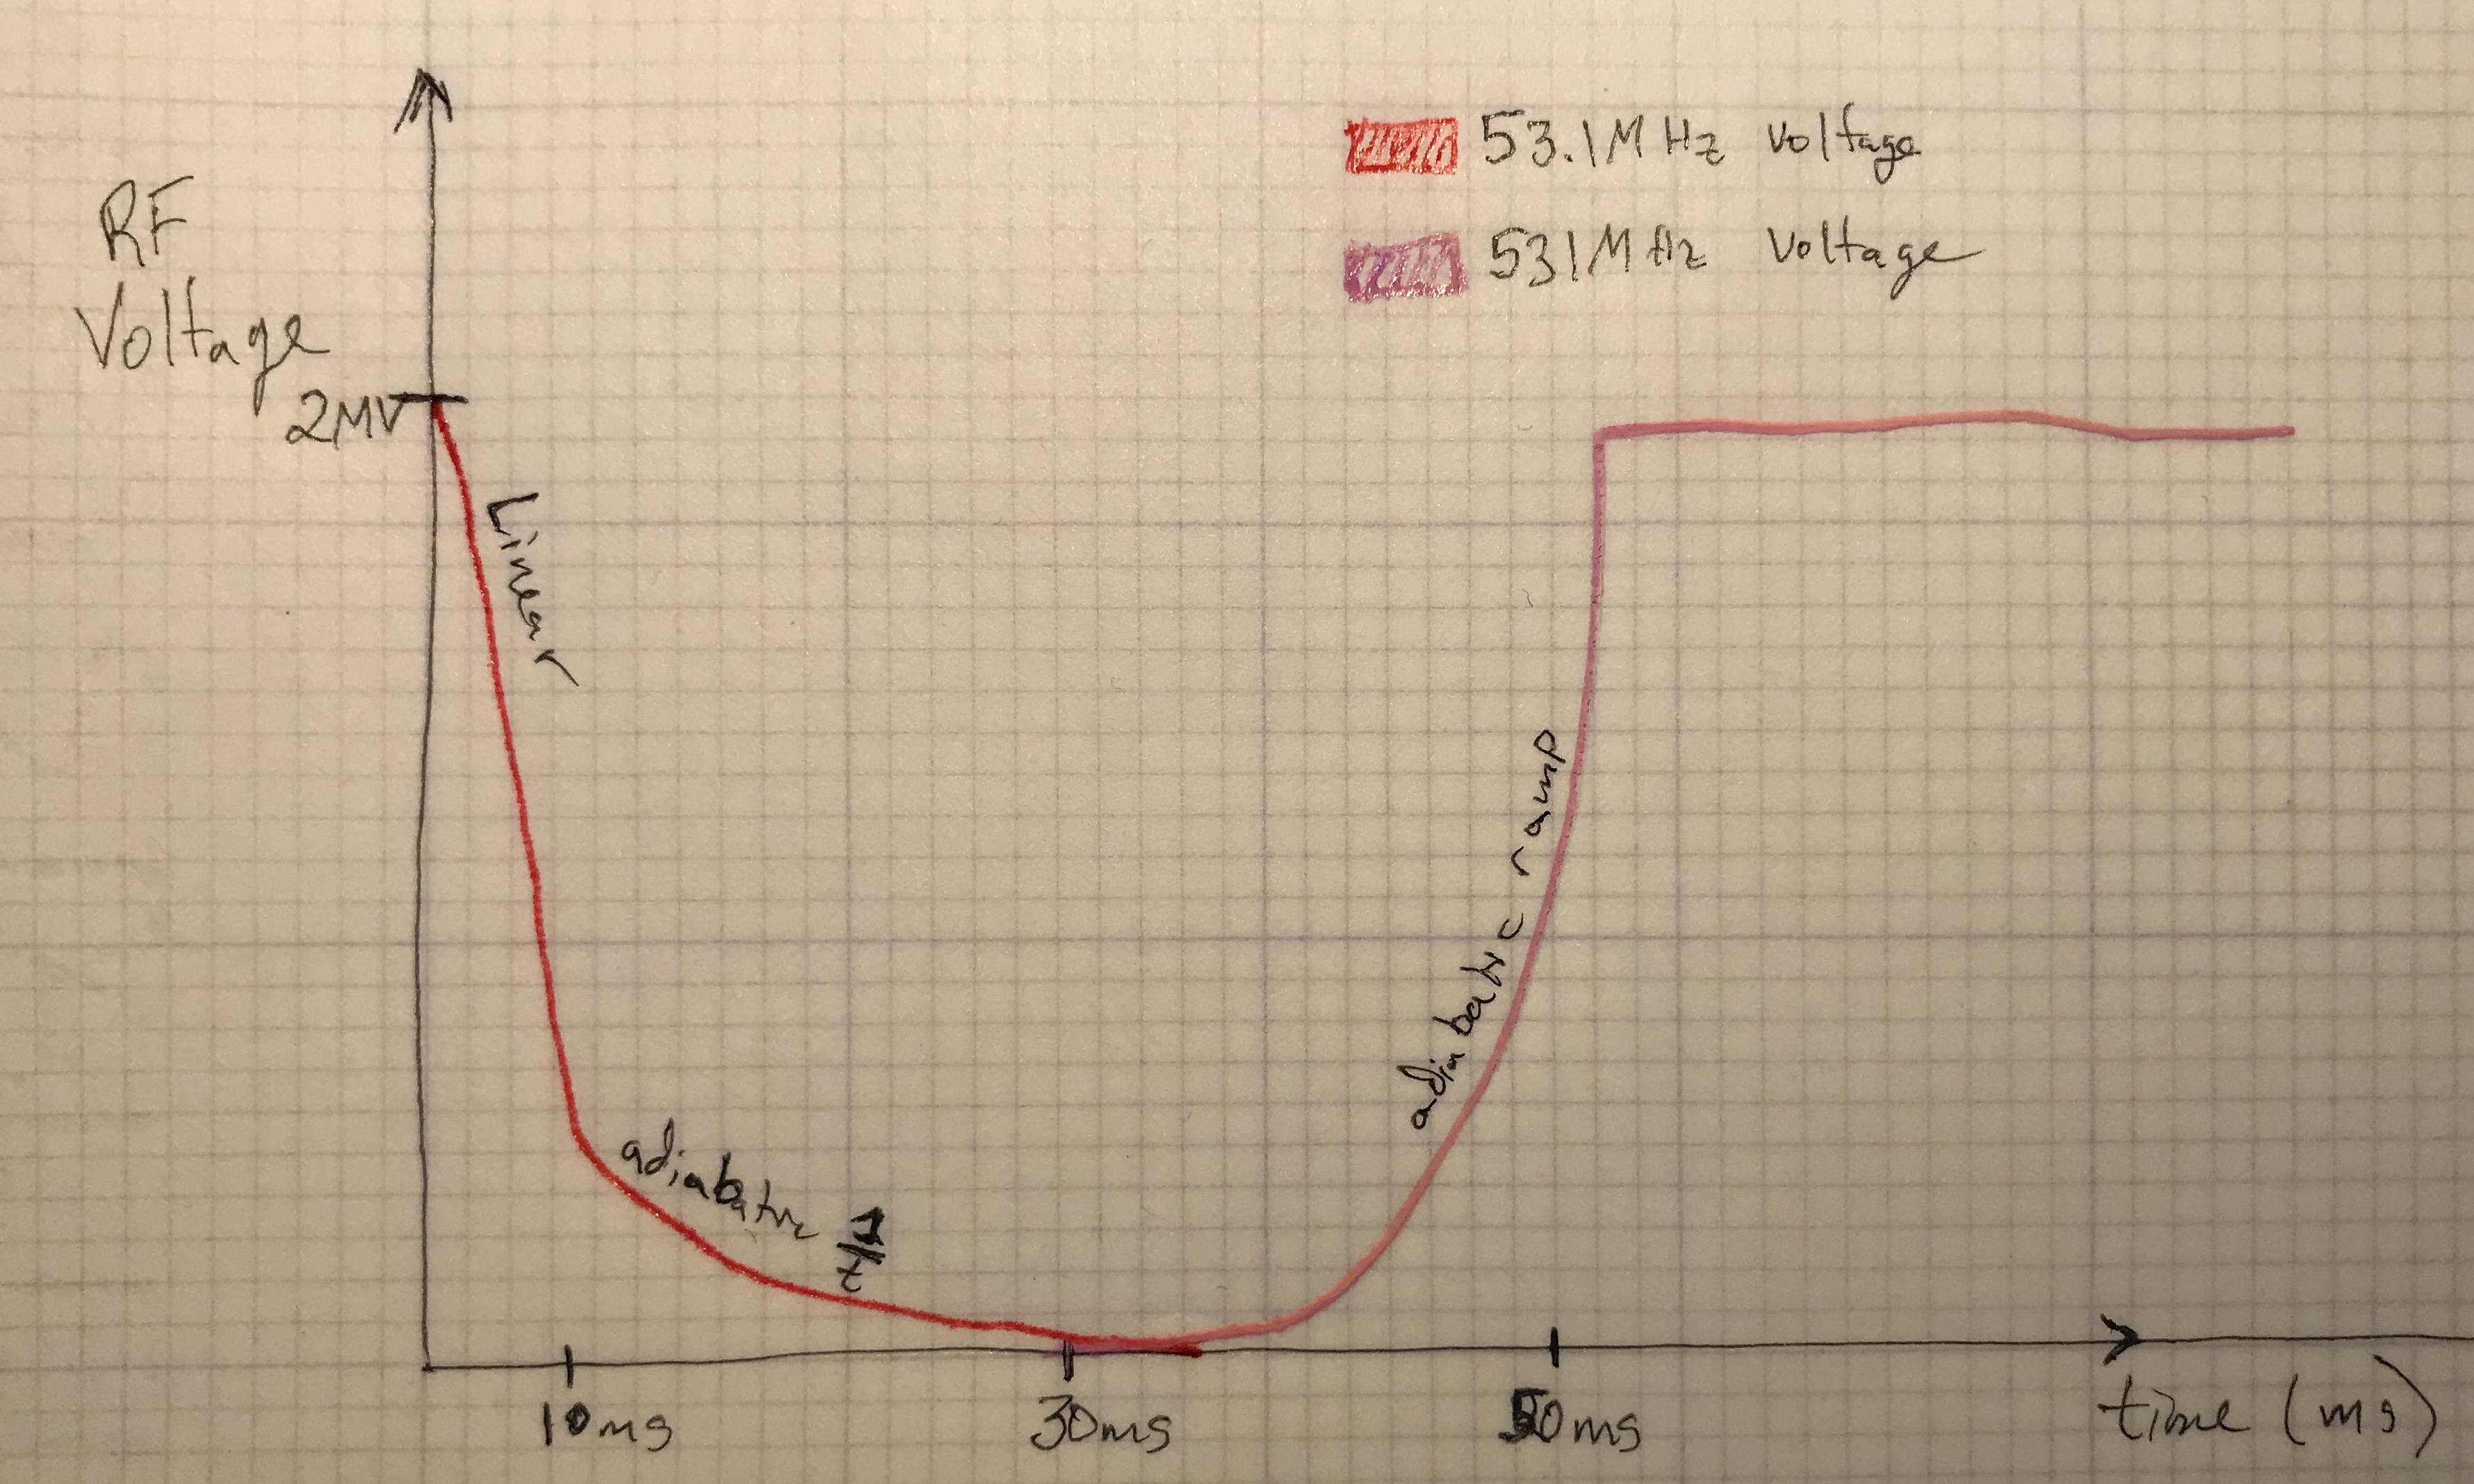
\includegraphics[width=0.60\linewidth]{Figures/draft_transition_voltages.JPG}
	\end{center}
	\caption{An example of the applied voltages to the 53.1MHz
          cavities (red) and the 531MHz cavity (pink). The 53.1MHz
          voltage function is a piece-wise function starting with
          linear decrease and then an adiabatic decrease using
          function *** down to 0 volts.}
		\label{fig:transition_voltages}
\end{figure}

\subsubsection{Results of one recipe for re-bunching}

Phase space distributions at various times are shown in figure
\ref{fig:bunch_distributions} for a simulation that takes the voltages
from figure \ref{fig:transition_voltages} as an input. The red
particles represent a best estimate of the present-day proton
distribution in the main injector before extraction.

\begin{figure}[t]
	\begin{center}
        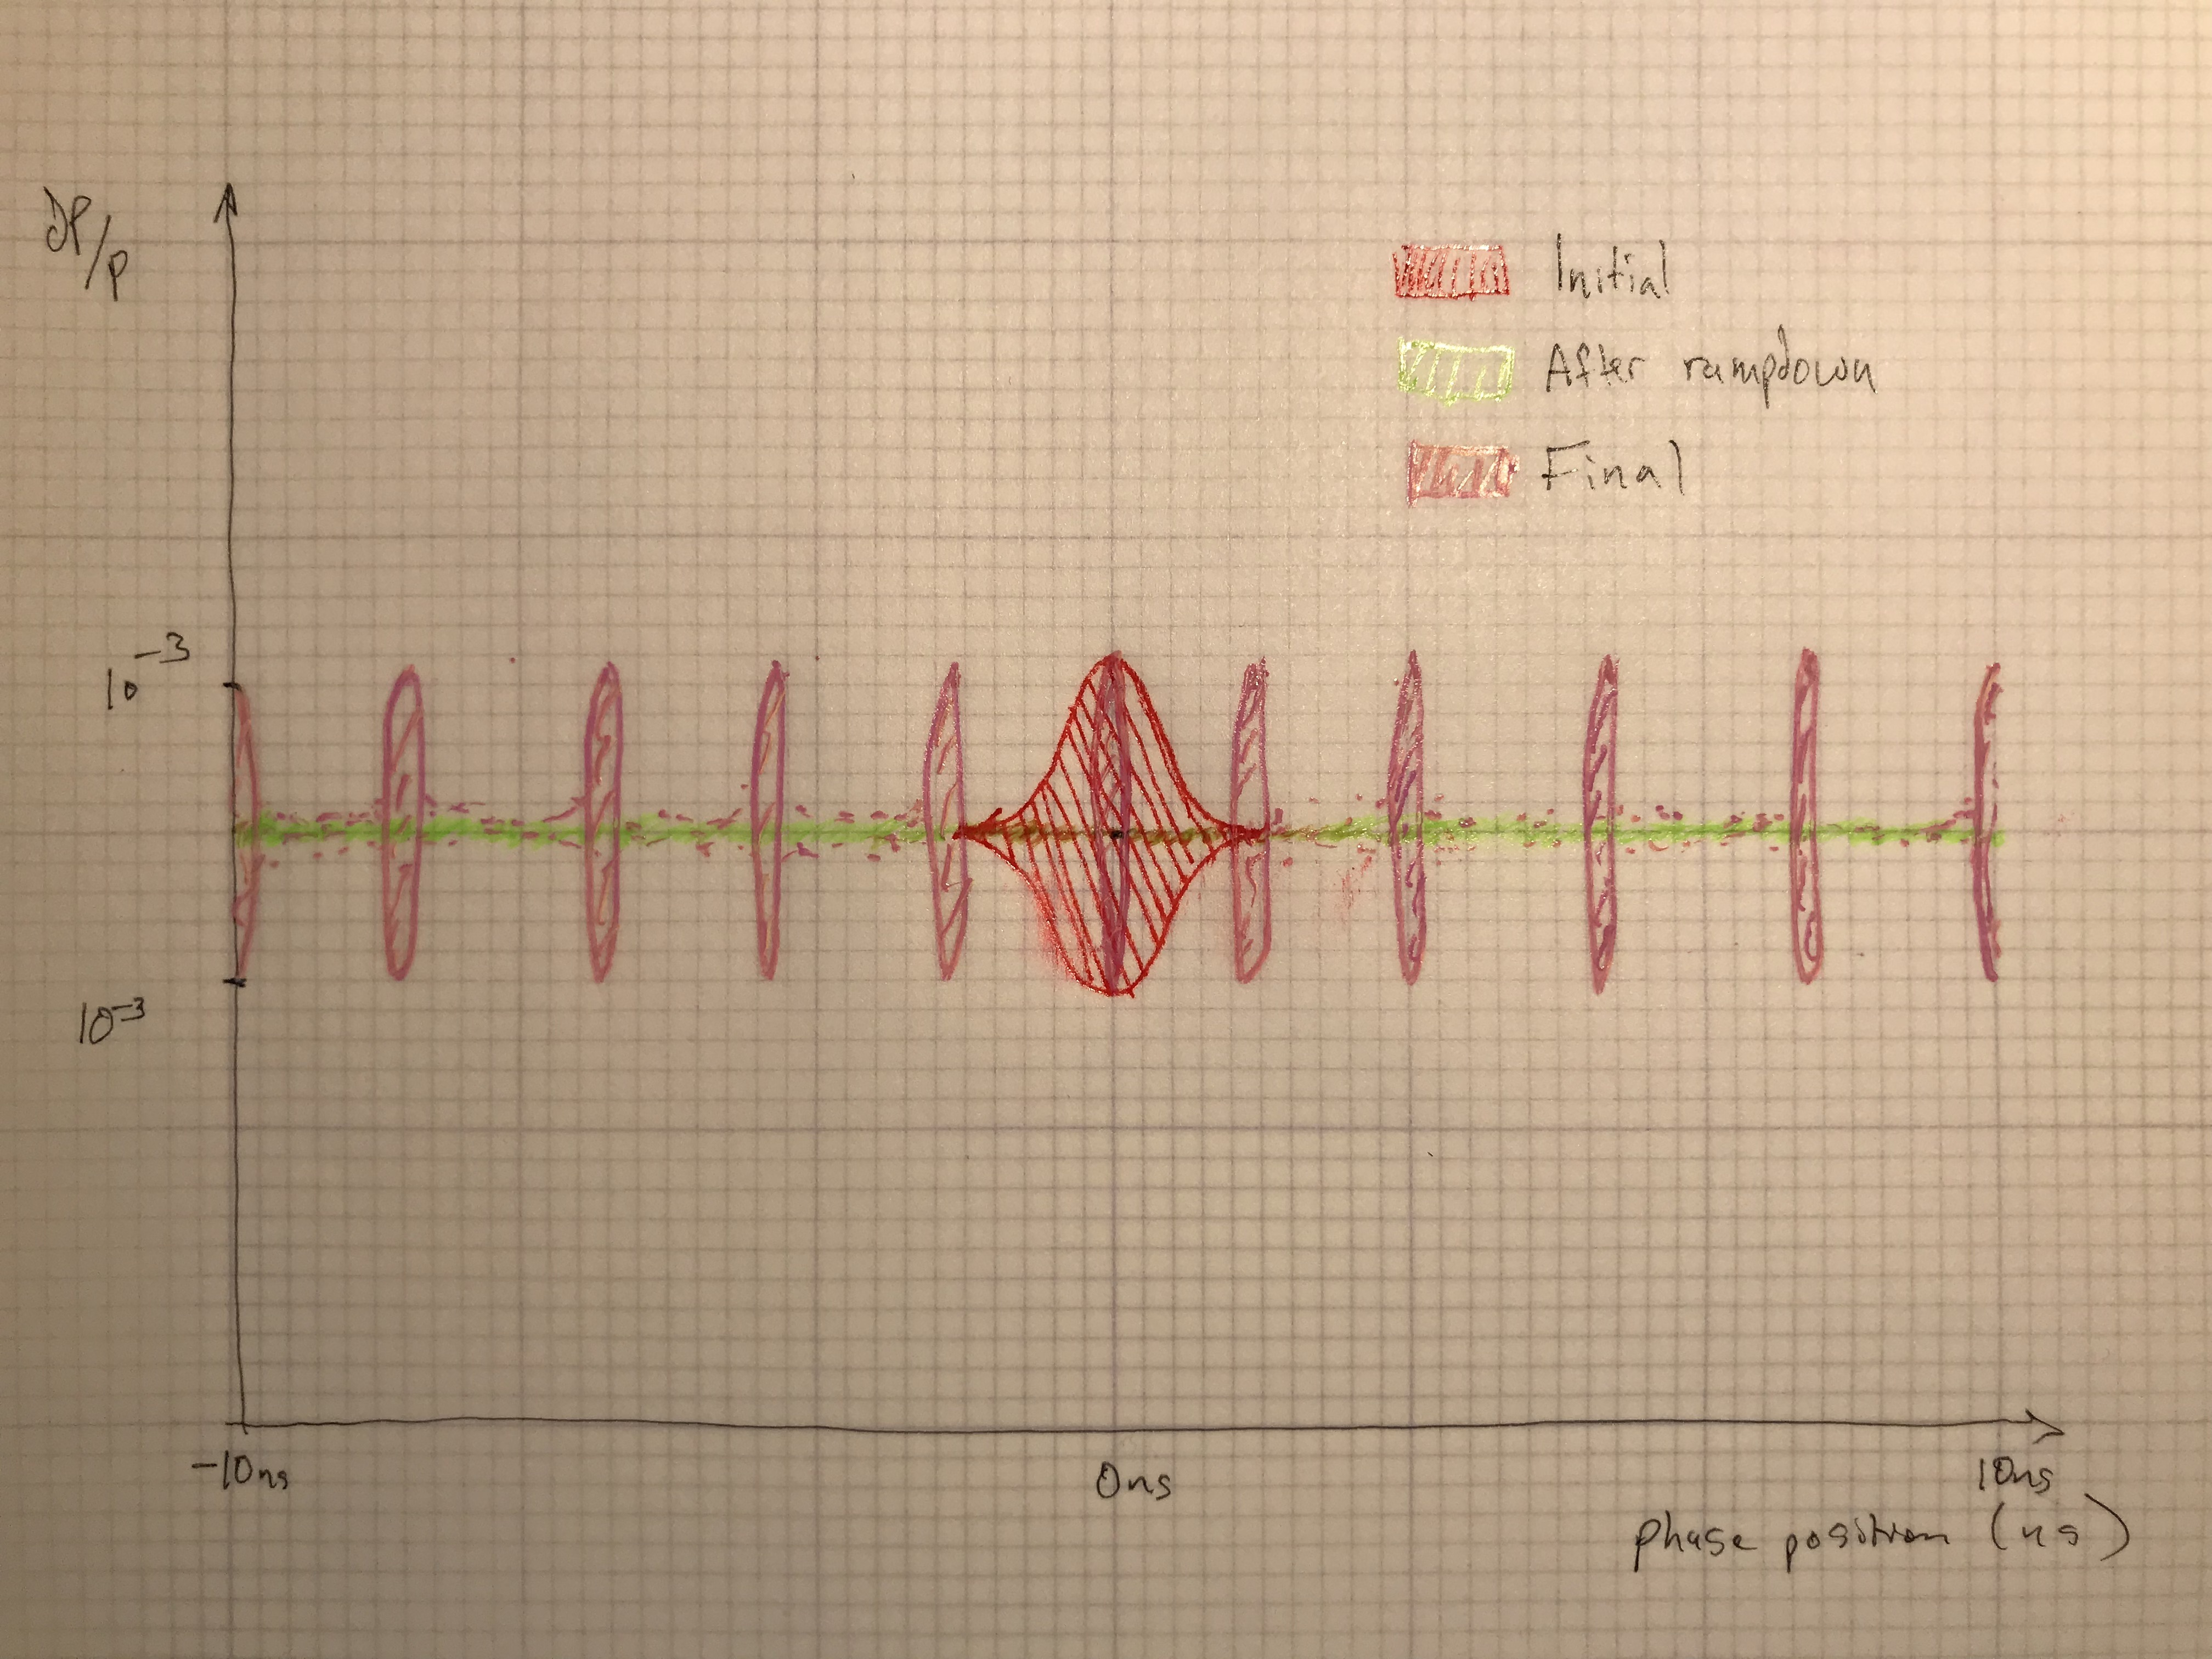
\includegraphics[width=0.60\linewidth]{Figures/draft_bunch_distributions.JPG}
	\end{center}
	\caption{Distribution of protons in energy spread vs. RF phase
          for the initial main injector proton bunch (red), the
          transition time between the two RF frequencies (green), and
          the end point after ramping the high frequency voltage
          (pink). This particular rebunching took a total of 50ms, a
          4\% addition to the total cycle time.}
		\label{fig:bunch_distributions}
\end{figure}

The objective of the rampdown of the 53.1 MHz voltage amplitude is to
create a thin line in $(\phi, \delta)$ phase-space. A thinner
distribution before applying higher frequency cavity voltage will lead
to smaller time-width bunches after the higher frequency cavity
voltage reaches 2 MV. An example of this thin-line transition point is
shown in green in figure \ref{fig:bunch_distributions}.

It has been observed that the final thin bunch RMS time-width is
relatively insensitive to the ramp-up time but highly sensitive to the
$\mathrm{d}p/p_0$ spread at the time of ramp-up (cite Evan's
technical/detailed write-up). The momentum spread at the transition
time is largely dictated by the ramp-down functions and their time
parameters. Therefore, the final time-width RMS was explored as a
function of total re-bunching time where the ramp-down time is varied.

Figure \ref{fig:bunch_width_curve} plots the final RMS time-width as a
function of the total re-bunch time divided by the main injector cycle
time. The fraction on the x-axis is equal to the loss in POT from
time-on-target alone.

\begin{figure}[t]
	\begin{center}
        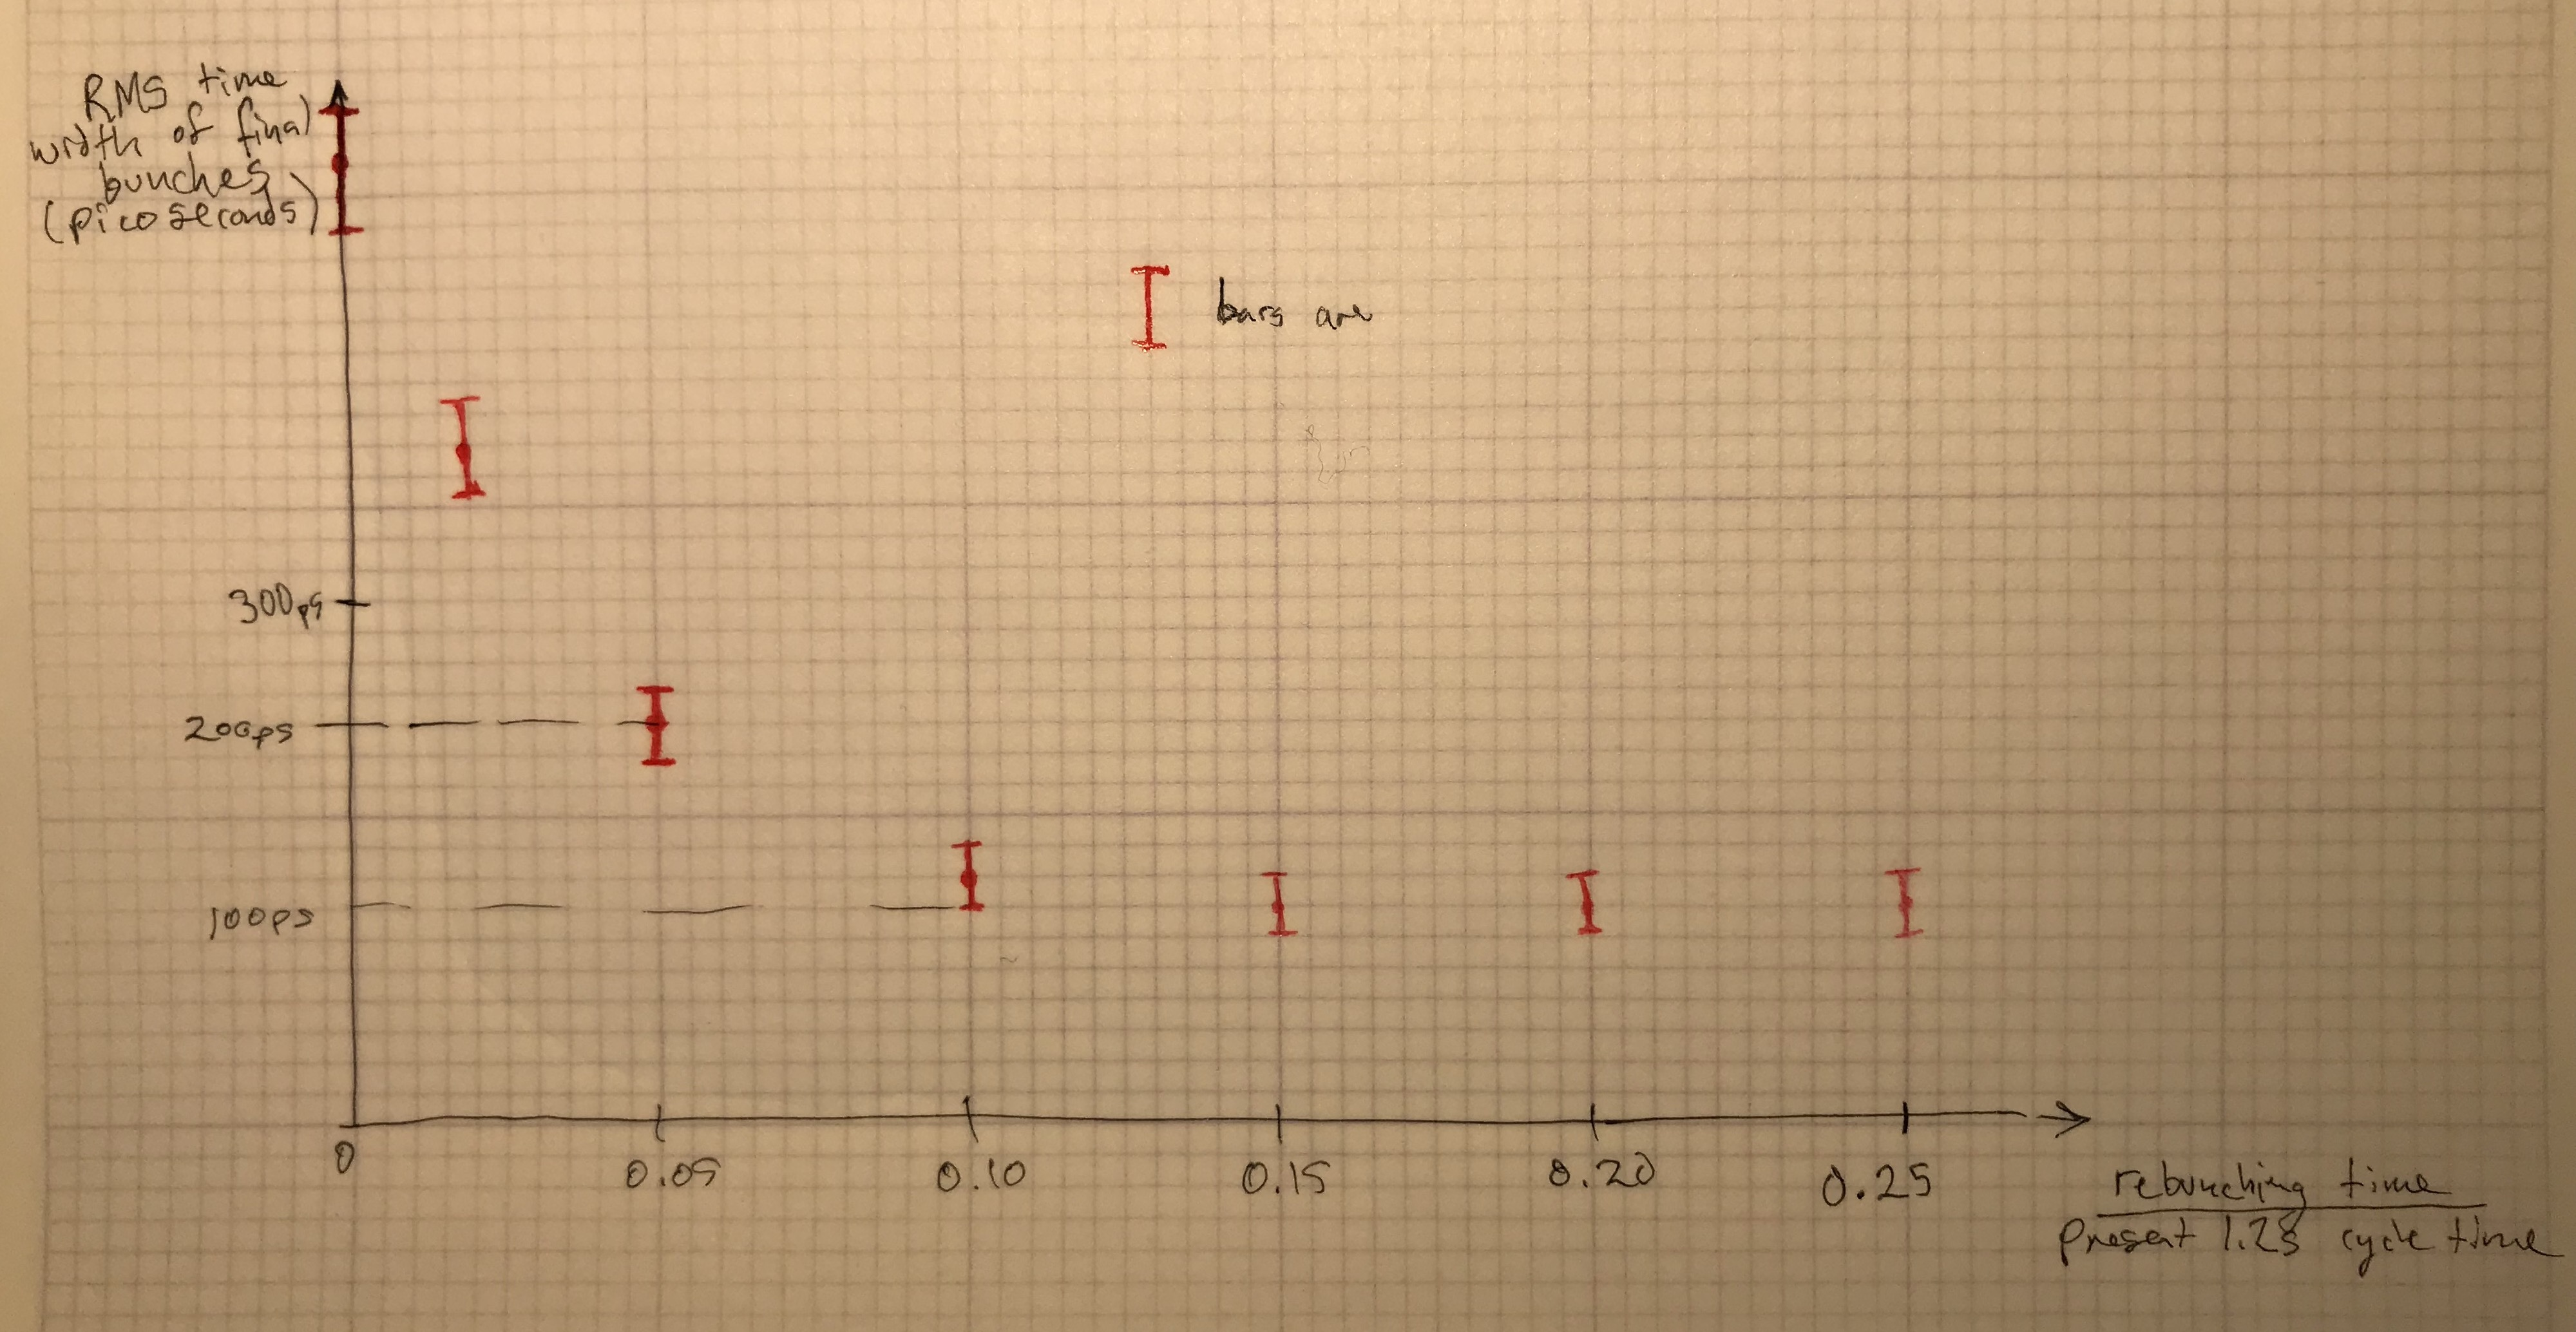
\includegraphics[width=0.60\linewidth]{Figures/draft_rms_vs_time.JPG}
	\end{center}
	\caption{The root-mean-square of the time distribution one of
          the thin, high-frequency bunches after going through a
          rebunching procedure that takes time $t$, where the x-axis
          is the ratio of $t$ to the present cycle time of $1.2$
          seconds. Longer re-bunching time corresponds to a reduction
          in POT because it increases the period between main injector
          dumps.}
		\label{fig:bunch_width_curve}
\end{figure}

This simulation shows that bunch widths on the order of 100 ps may be
achieved given a single RF cavity at about 500 MHz and the properly
optimized voltage functions for re-bunching without too much more than
5\% loss in POT.

% End of Section 6
